\section{Introduction}

    \subsection{Cahier des charges}

        \begin{frame}
            \frametitle{Cahier des charges et objectifs}
            \begin{block}{Intitulé du sujet}
                Lecture en clair, grâce à l'utilisation de la réalité augmentée, d'oeuvres réelles préalablement chiffrées et imprimées.
            \end{block}

            \begin{exampleblock}{Conditions}
                \begin{itemize}
                    \item Documentation, définition des niveaux de précision
                    \item Développement itératif
                    \item Comprendre, appliquer nous-même
                \end{itemize}
            \end{exampleblock}
        \end{frame}

    \subsection{Étude bibliographique}

        \begin{frame}
            \frametitle{Méthodes de chiffrement}
            \framesubtitle{Chiffrement symétrique}
            \centering{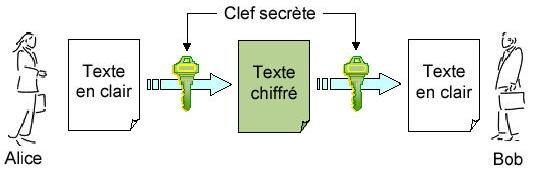
\includegraphics[width=.8\linewidth]{rsc/symetrique.png}}
            \blfootnote{http://igm.univ-mlv.fr/~dr/XPOSE2007/vma\_PKI/concepts\_de\_base.html}
        \end{frame}

        \begin{frame}
            \frametitle{Méthodes de chiffrement}
            \framesubtitle{Chiffrement asymétrique}
            \begin{columns}
                \begin{column}{.4\linewidth}
                    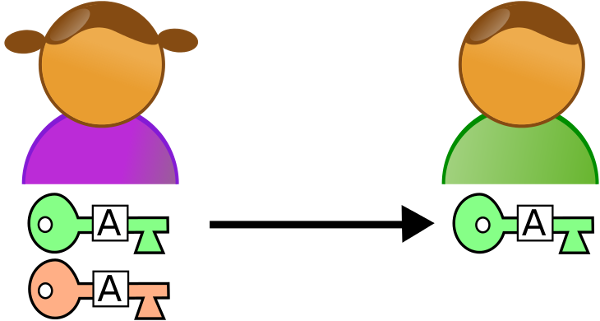
\includegraphics[width=\linewidth]{rsc/asymetrique_1.png}
                \end{column}

                \begin{column}{.4\linewidth}
                    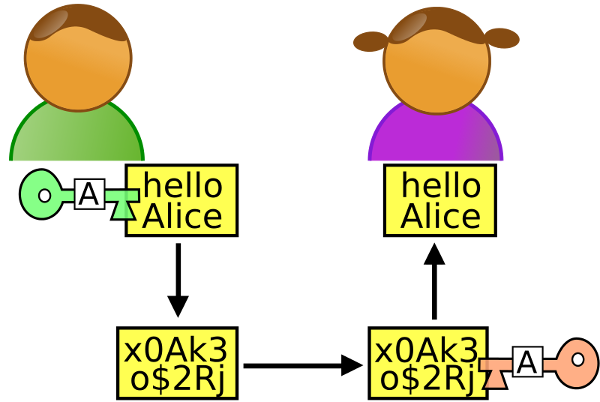
\includegraphics[width=\linewidth]{rsc/asymetrique_2.png}
                \end{column}
            \end{columns}
            \blfootnote{https://fr.wikipedia.org/wiki/Cryptographie\_asymétrique}
        \end{frame}

        \begin{frame}
            \frametitle{Méthodes de chiffrement}
            \framesubtitle{Chiffrement asymétrique avec authentification}
            \centering{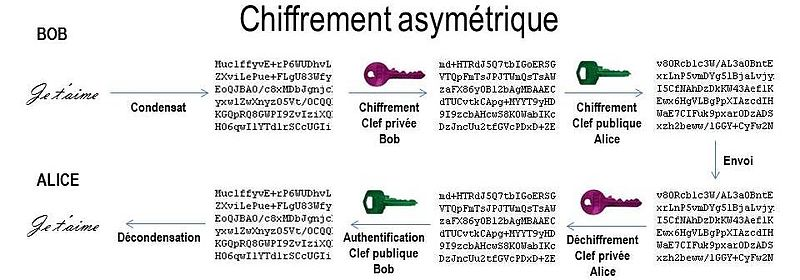
\includegraphics[width=.8\linewidth]{rsc/authentification.png}}
            \blfootnote{https://fr.wikipedia.org/wiki/Cryptographie\_asymétrique}
        \end{frame}

        \begin{frame}
            \frametitle{Techniques de chiffrement}
            \begin{columns}
                \begin{column}{.4\linewidth}
                    \centering{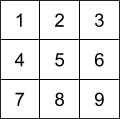
\includegraphics[width=.6\linewidth]{rsc/tab_base.png}}\\
                    \pause
                    \centering{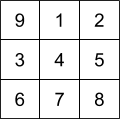
\includegraphics[width=.6\linewidth]{rsc/tab_permutation.png}}
                    \pause
                    \begin{columns}
                        \begin{column}{.5\linewidth}
                            \textcolor{green}{+ ca c'est bien}
                        \end{column}

                        \begin{column}{.5\linewidth}
                            \textcolor{red}{- ca c'est pas bien}
                        \end{column}
                    \end{columns}
                \end{column}

                \begin{column}{.4\linewidth}
                    \pause
                    \centering{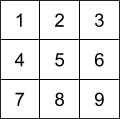
\includegraphics[width=.6\linewidth]{rsc/tab_base.png}}\\
                    \pause
                    \centering{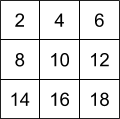
\includegraphics[width=.6\linewidth]{rsc/tab_substitution.png}}
                    \pause
                    \begin{columns}
                        \begin{column}{.5\linewidth}
                            \textcolor{green}{+ ca c'est bien}
                        \end{column}

                        \begin{column}{.5\linewidth}
                            \textcolor{red}{- ca c'est pas bien}
                        \end{column}
                    \end{columns}
                \end{column}
            \end{columns}
        \end{frame}

        \begin{frame}
            \frametitle{Exemple d'algorithmes}
            \begin{columns}
                \begin{column}{.3\linewidth}
                    \begin{center}
                        AES (année)\\
                        technique?\\
                        efficace?
                    \end{center}
                \end{column}

                \begin{column}{.3\linewidth}
                    \begin{center}
                        DES (année)\\
                        technique?\\
                        efficace?
                    \end{center}
                \end{column}

                \begin{column}{.3\linewidth}
                    \begin{center}
                        RSA (année)\\
                        technique?\\
                        efficace?
                    \end{center}
                \end{column}
            \end{columns}

            \begin{columns}
                \begin{column}{.45\linewidth}
                    \begin{center}
                        arnold (année)\\
                        technique?\\
                        efficace?
                    \end{center}
                \end{column}

                \begin{column}{.45\linewidth}
                    \begin{center}
                        queue (année)\\
                        technique?\\
                        efficace?
                    \end{center}
                \end{column}
            \end{columns}
        \end{frame}
